\documentclass{article}
\usepackage[utf8]{inputenc}
\usepackage[margin=3cm]{geometry}
\usepackage{indentfirst}
\usepackage{graphicx}
\usepackage{amsmath}
\graphicspath{ {./images/} }
\setlength{\parindent}{0.75cm} %heh, 0.75

\title{
    \textbf{Programação 3D - Assignment I}
    }
\author{
    \begin{Large}
        \textbf{Grupo 02}
    \end{Large}\\
    Francisco Campaniço 83463\\
    João Rafael 83482\\
    Rodrigo Oliveira 83558
}
\date{Março 2019}

\begin{document}

    \maketitle

    \section*{\textit{Parser} NFF}

        \par 
        O programa começa por ler o ficheiro NFF definido pelo utilizador no início do código. Seguindo a especificação do formato NFF, adiciona uma câmara, luzes e objetos à cena. A cena (classe \texttt{Scene}) contêm uma câmara, um número de luzes definido pelo ficheiro NFF, e objetos também definidos pelo mesmo.
        \par
        Um objeto (classe \texttt{SceneObject}) contém uma classe \texttt{Material} e métodos genéricos de interseção e cálculo de normais, que são \textit{overriden} pelas classes que herdam desta.
        \par
        Dado que o formato NFF não têm uma opção para \textit{Bounding Boxes}, foi adicionada uma opção para tal: \texttt{aabb x0 x1 y1 y2 z1 z2}, que cria uma AABB com os limites em cada eixo declarados pelas variáveis seguintes.

    \section*{Interseções}

        \par
        O raio verifica interseções com objetos ao chamar o método \texttt{intersect} de cada objeto, que devolve um \textit{boolean} e a distância \textit{t} da origem do raio ao objeto. Depois disto, o objeto com menor \textit{t} é o mais próximo, logo os cálculos seguintes de iluminação aplicam-se a este.

        \par
        A tabela abaixo contém os resultados de tempo para cada um dos testes disponibilizados. Estes resultados foram obtidos num portátil com um CPU Intel Core i7-8750H (6 \textit{cores}, 2.2GHz) e uma GPU NVIDIA GTX 1060, correndo Kubuntu 18.04 e usando o programa Unix \texttt{time} para determinar o tempo de execução.

        \begin{table}[h]
            \centering
            \begin{tabular}{|l|l|l|l|l|}
                \hline
                Teste & Low     & Medium    & High     & Very High \\ \hline
                Balls & 0m11s   & 0m18s     & 12m14s   & -         \\ \hline
                Mount & 0m15s   & -         & 8m58s    & 2h21m3s   \\ \hline
            \end{tabular}
        \end{table}
    \subsection*{Raio - Esfera}

        \par
        O cálculo da interseção raio - esfera contém várias otimizações. Primeiro, se a distância entre a origem do raio e o centro da esfera for maior que o raio da mesma, calcula-se 
        $$ B = x_d (x_c + x_o) + y_d (y_c + y_o) + z_d (z_c + z_o). $$
        Se B for negativo, o raio aponta para a direção oposta da esfera pode-se concluir que não há interseção.
        \par
        Depois, calculamos $$ R = B^2 - C = B^2 - d^2_{OC} + r^2 $$ e se B for negativo, conclui-se também que não há interseção.
        \par
        Finalmente, concluimos que há interseção, e calculamos
        $$
            t_i =
            \begin{cases}
                B - \sqrt{R}, &\mbox{se } d^2_{OC} > r^2\\
                B + \sqrt{R}, &\mbox{se } d^2_{OC} \leq r^2 
            \end{cases}
        $$
        para determinar o ponto de interseção e a sua normal, para efeitos de cálculo de cor.
        

    \subsection*{Raio - Plano}
        \par
        A interseção raio - plano é simples; calcula-se o produto interno da normal do plano e a direção do raio. Se esta for zero, o raio e o plano são paralelos e como tal não se podem intersetar.
        \par
        Depois, calculamos
        $$
            t_i = -\frac{(o - a) \cdot n }{ n \cdot d}.
        $$
        Se $t$ for negativo, rejeita-se os cálculos. Caso contrário, usa-se o $t$ para determinar o ponto de interseção e a sua normal.
    \subsection*{Raio - Triângulo}

        \par
        Para calcular a interseção entre raios e triânglos, utiliza-se o algoritmo de Möller-Trumbore. Primeiro, calculamos o determinante da matriz com os 3 pontos do polígono, que também pode ser calculada através de 
        $$
            det = a_{01} \cdot (d \times a_{02} ),
        $$
        $a_{01}$ e $a_{02}$ sendo arestas do triângulo. Se este determinante for zero, raio e triângulo são paralelos e abandonam-se os cálculos de interseção.
        \par
        Depois, calcula-se coordenadas baricêntricas $u$ e $v$. Se $u$ não estiver no intervalo (0,1), $v$ for negativo ou $u + v > 1$, abandonam-se os cálculos.
        \par
        Finalmente, calculamos
        $$
            t_i = \frac{1}{det} (a_{02} \cdot ((o -v_0) \times a_{01})).
        $$
        Se $t$ for negativo, a direção do raio é oposta ao vetor entre raio e triângulo, por isso abandonam-se os cálculos. Caso contrário, há uma interseção e usamos $t$ para calcular o ponto de interseção e a normal correspondente.

    \subsection*{Raio - Cone (Extra)}
        \begin{center}
            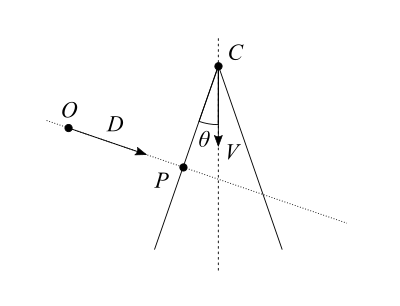
\includegraphics[scale=0.60]{cone}
        \end{center}
        \par
        Começamos por descobrir o valor do seno e coseno de $ \theta $ através de V, C e P. Depois calculamos os valores de a,b e c de acordo com a fórmula quadrática
        $ at^2 + bt + c = 0 $:
        \begin{equation*}
            \begin{cases}
                a &= (\overrightarrow{D} \cdot \overrightarrow{V})^2 - cos^2 \theta \\
                b &= 2(\overrightarrow{D} \cdot \overrightarrow{V})(\overrightarrow{C}O \cdot \overrightarrow{V}) - \overrightarrow{D} \cdot \overrightarrow{C}O cos^2 \theta \\
                c &= (\overrightarrow{C}O \cdot \overrightarrow{V})^2 - \overrightarrow{C}O \cdot \overrightarrow{C}O cos^2 \theta \\
            \end{cases}
        \end{equation*}
        De seguida calculamos o determinante $\Delta = b^2 - 4ac$ e discartamos os casos em que este é menor ou igual a zero. No caso de ser maior apenas 
        rejeitamos o t que está no lado da sombra e vemos se este é menor que uma constante muito pequena. Caso seja maior devolvemos que o raio interseta o cone.
    \subsection*{Raio - AABB (Extra)}
        % br pls
    \section*{Iluminação Blinn-Phong}
        \par
        Para calcular a cor dos pixeis de acordo com as luzes da cena usamos o modelo de iluminação Blinn-Phong, isto é, começamos com a normal, 
        o vetor que vai do ponto até à fonte de luz e calculamos a sua distância e, por consequência, a atenuação, visto que as luzes são todas 
        \textit{point lights}. Depois faz-se o produto interno entre a normal e o vetor que foi calculado previamente para se encontrar a intensidade e, por fim, 
        as descrições do material para encontrar a componente difusa.
        \par
        Falta só calcular a componente especular e para isso usamos o \textit{half vector}, que é a soma do vetor de direção da luz com o \textit{view vector} e
        com isso efetuamos o mesmo calculo usado para a componente difusa e ficamos com a componente especular.
        \par
        Finalmente usamos as duas componentes calculadas e as descrições dos materiais para encontrar a cor do raio respetivo. Com múltiplas luzes apenas basta somar o resultado 
        desta função com todas as luzes da cena e usando o fator de sombra que vai ser explicado a seguir.
    \section*{Sombras}
        \par
        Para calcular as sombras começamos por descobrir o vetor de direção da luz em relação ao ponto em questão e
        depois criamos um raio com origem no ponto mais a direção da luz e com essa direção. Finalmente descobre-se a interseção deste raio com os objetos da cena (como 
        fosse um raio normal) e, caso este intersete um objeto, a função devolve um valor lógico positivo.
        \par
        Este valor vai ser usado depois para determinar se o valor devolvido é 0 ou 1 (1 caso tenha intersetado algum objeto), para que depois se possa 
        multiplicar o simetrico desse valor na componente de cor devolvida pelo calculo de Blinn-Phong.
    \section*{Reflexão}
        \par
        Para calcular a reflexão começamos por ver se o material do objeto é refletor (componente especular maior que 0). Depois calculamos o raio refletor da seguinte forma:
        \begin{equation*}
            \begin{split}
                &p(t) = p_i + t\hat{r}_r.\\
                &\textrm{onde,}\\
                &\hat{r}_r = 2(V \cdot \hat{n})\hat{n} - V \\
                &V_n = (V \cdot \hat{n})\hat{n}\\
                &h = V_n - n \\
                &\hat{r}_r = V_n + h
            \end{split}
        \end{equation*}
        \par
        Finalmente basta calcular a cor deste novo raio através do algoritmo de \textit{ray tracing} e depois somá-la à cor já previamente obtida.
        \begin{center}
            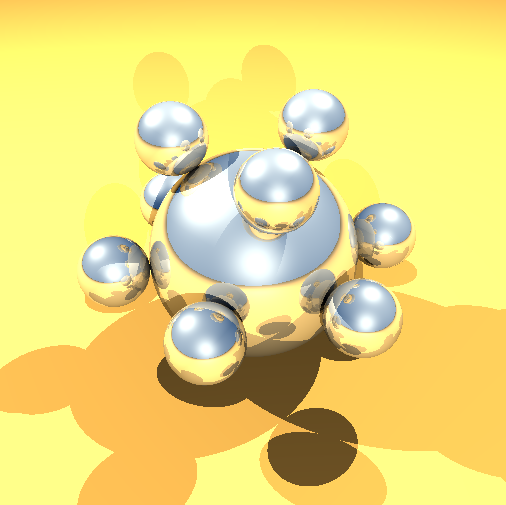
\includegraphics[scale=0.27]{deez_low}
            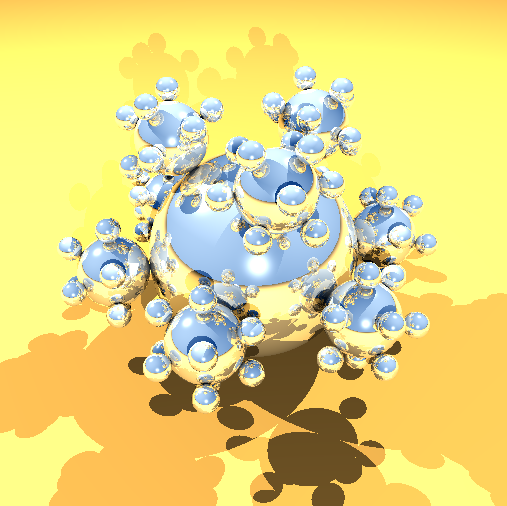
\includegraphics[scale=0.27]{deez_med} 
            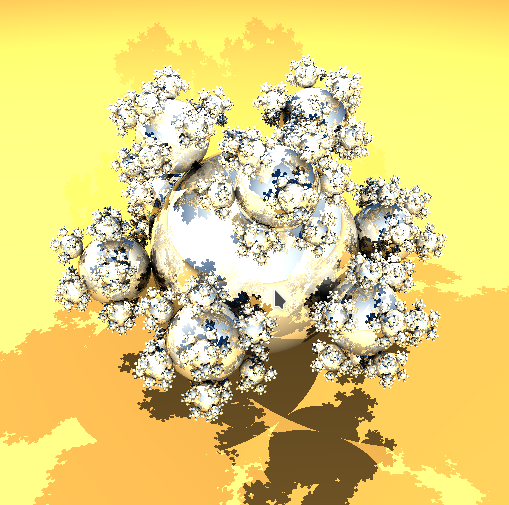
\includegraphics[scale=0.27]{deez_high} 
        \end{center}

    \section*{Refração}
        % br pls
        \begin{center}
            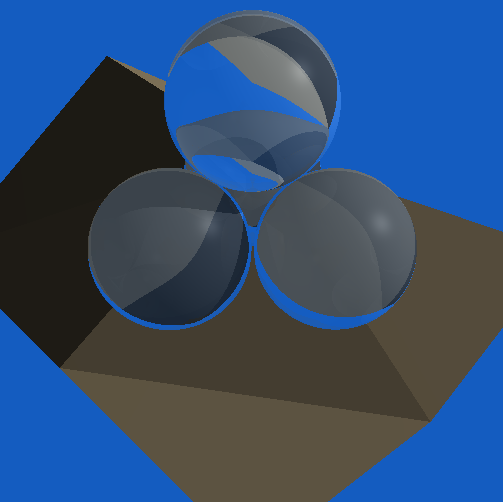
\includegraphics[scale=0.27]{mount_low}
            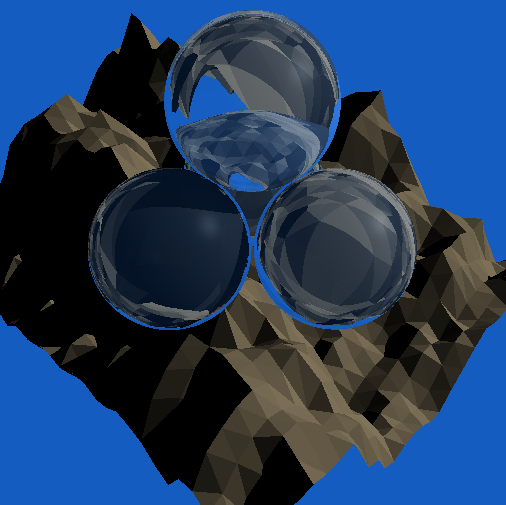
\includegraphics[scale=0.27]{mount_med} 
            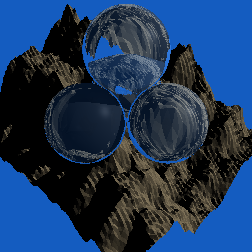
\includegraphics[scale=0.54]{mount_high} 
        \end{center}

\end{document}
